\documentclass{standalone}
\usepackage{tikz}
\usepackage{amsmath}
\usetikzlibrary{automata, positioning, arrows.meta}

\begin{document}
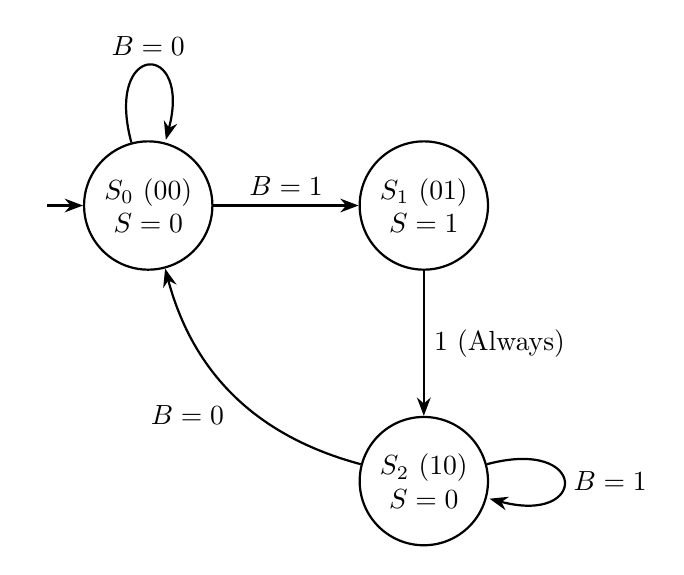
\begin{tikzpicture}[>=Stealth, node distance=3.5cm, on grid, auto, thick, initial text=]
    % States
    \node[state, initial, align=center] (S0) {$S_0$ (00) \\ $S=0$};
    \node[state, align=center] (S1) [right=of S0] {$S_1$ (01) \\ $S=1$};
    \node[state, align=center] (S2) [below=of S1] {$S_2$ (10) \\ $S=0$};

    % Transitions
    \path[->]
        (S0) edge [loop above] node {$B=0$} (S0)
             edge node {$B=1$} (S1)
        (S1) edge node [align=left] {1 (Always)} (S2)
        (S2) edge [loop right] node {$B=1$} (S2)
             edge [bend left] node {$B=0$} (S0);
\end{tikzpicture}
\end{document}
